\section*{Autores}

\begin{wrapfigure}{l}{0.3\linewidth}
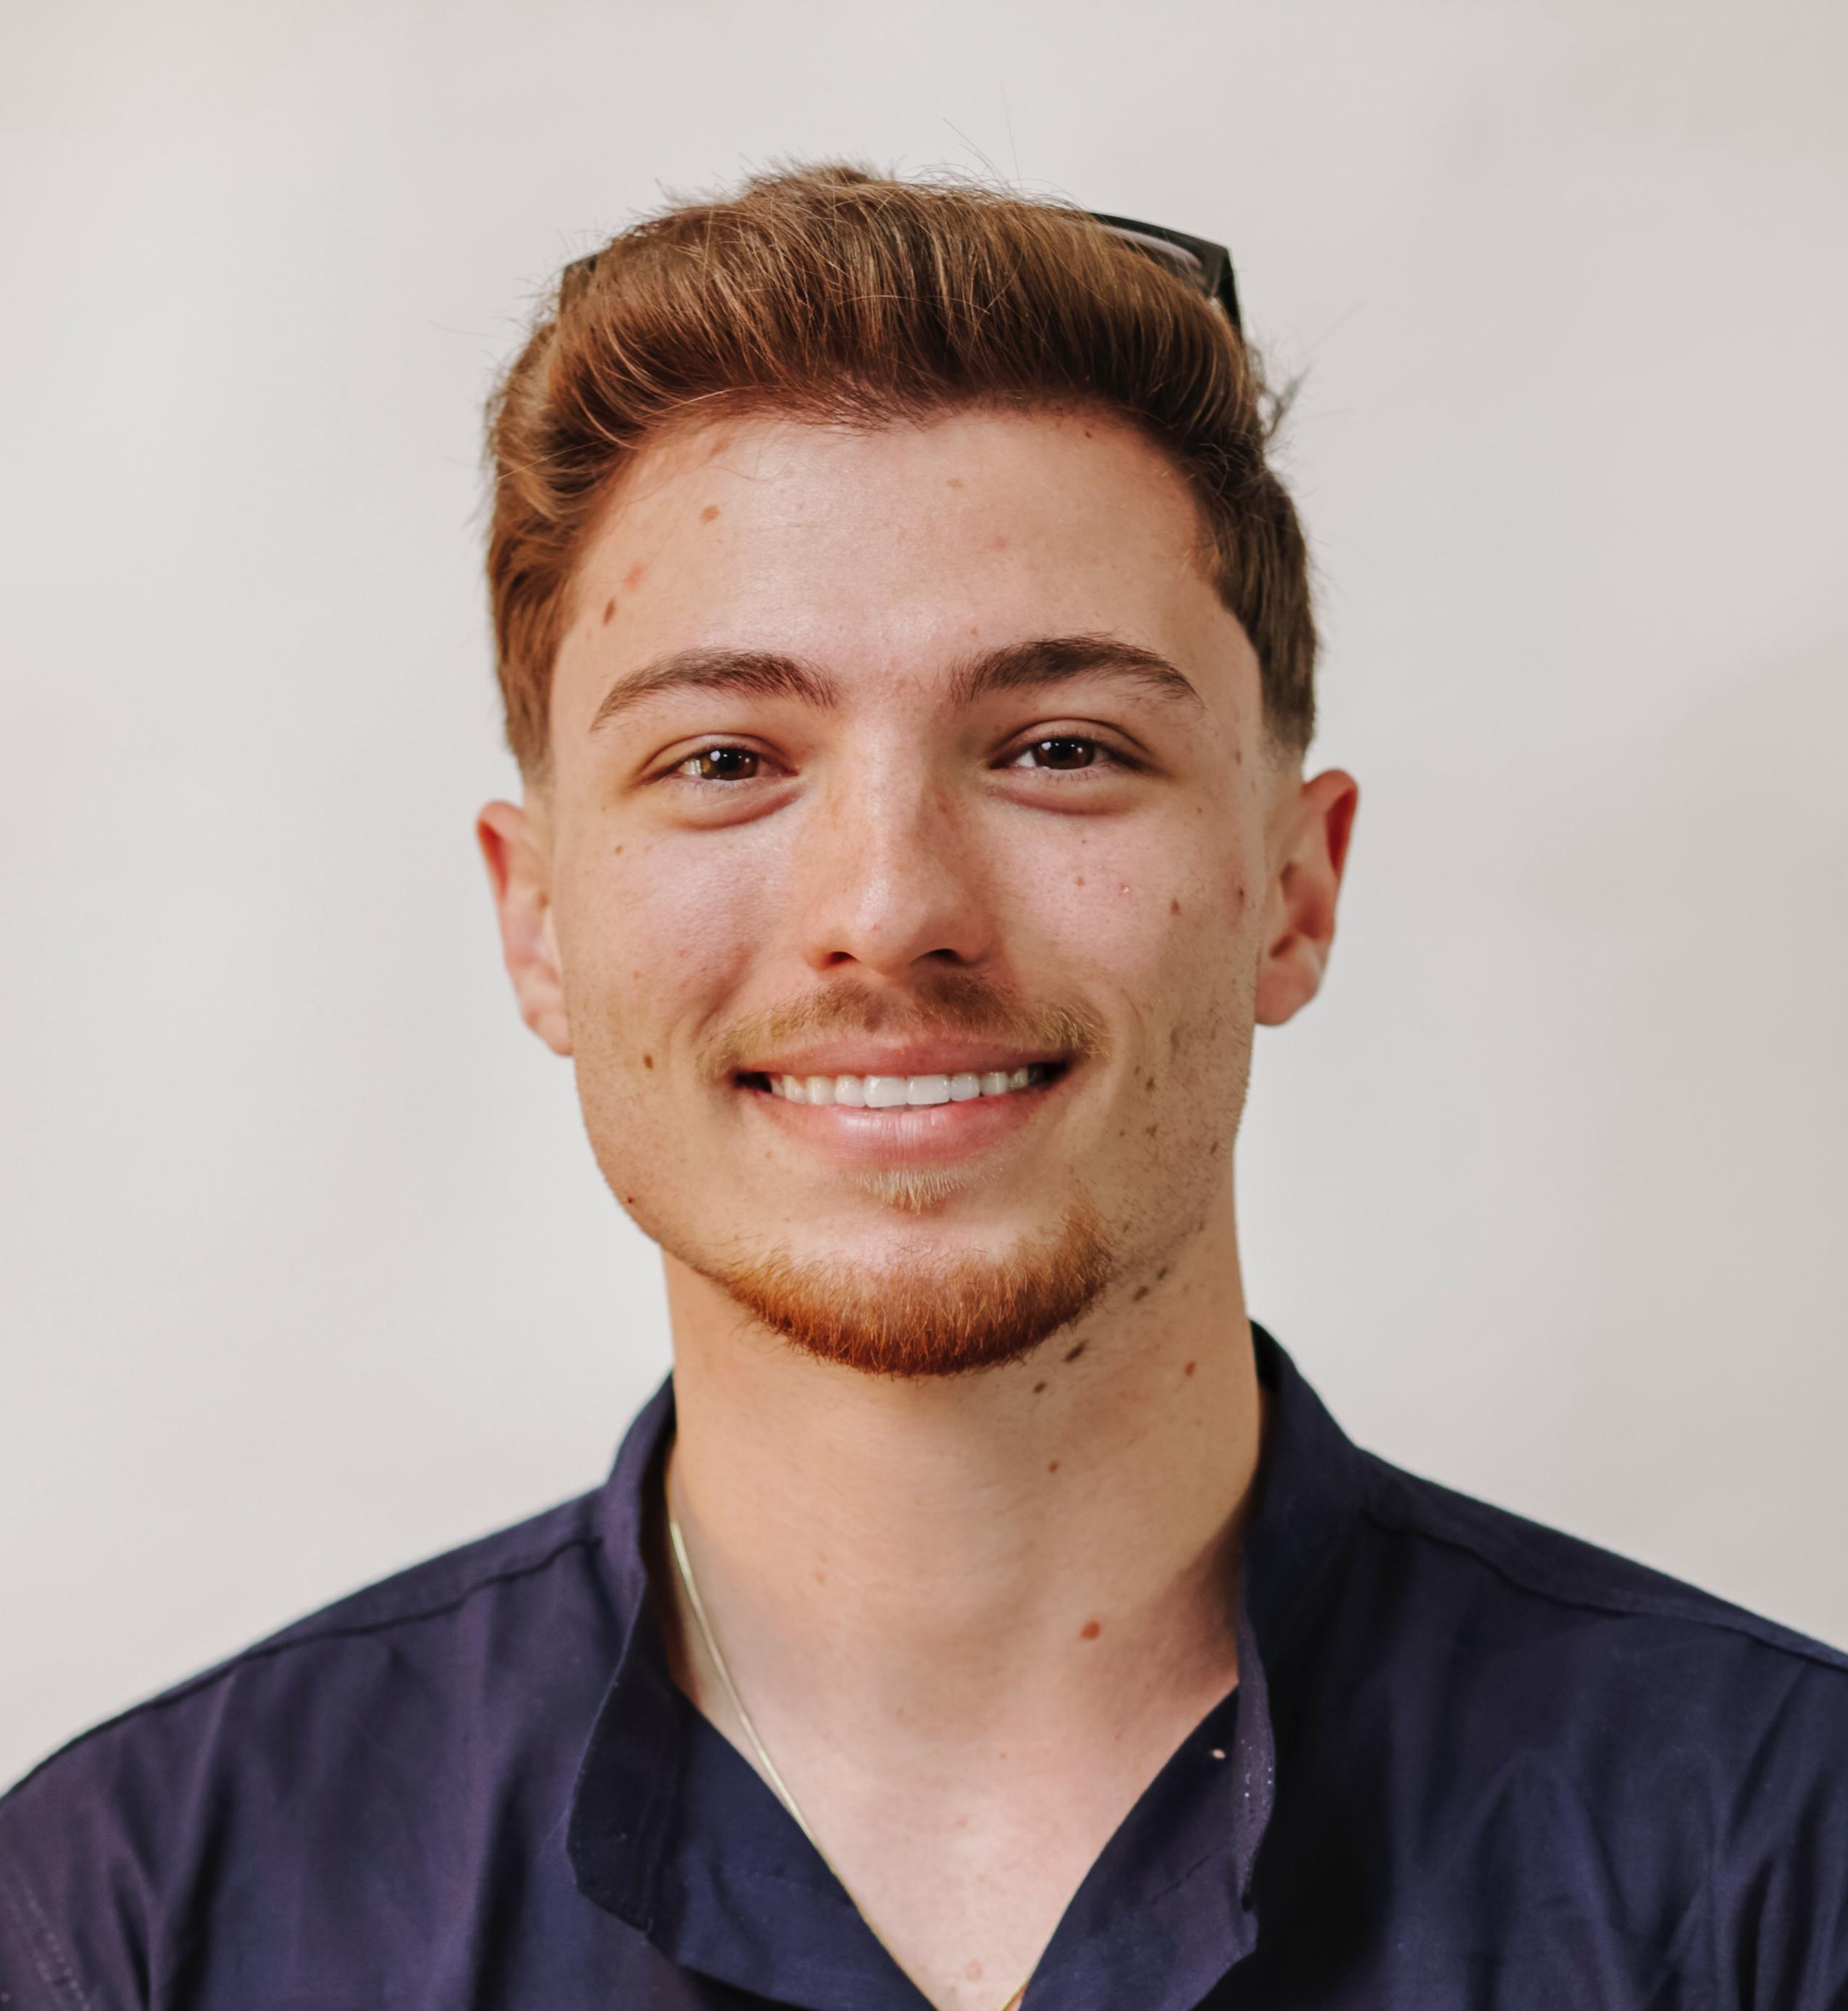
\includegraphics[width=\linewidth]{figuras/dimitri.jpeg}
\end{wrapfigure}

    \textbf{Dimitri Schulz Amado} é graduando em Engenharia de Software pelo Instituto Nacional de Telecomunicações (Inatel), com previsão de conclusão em 2026. Atua na area de desenvolvimento de software com foco em backend e infraestrutura. Possui experiência e tem interesse nas áreas da Engenharia de Software e DevOps.
    \newline

\begin{wrapfigure}{l}{0.3\linewidth}
\includegraphics[width=\linewidth]{figuras/Zeca.jpeg}
\end{wrapfigure}

    \textbf{José Carlos Rebouças Neto} é graduando em Engenharia de Software pelo Instituto Nacional de Telecomunicações (Inatel), com previsão de conclusão em 2026. Atua na área de desenvolvimento de software com foco em backend com comunicação em tempo real, utilizando tecnologias como React Native e WebSocket. Possui interesse em Engenharia de Software e Qualidade de Software.
    \newline

\begin{wrapfigure}{l}{0.3\linewidth}
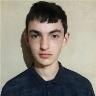
\includegraphics[width=\linewidth]{figuras/pedro.jpeg}
\end{wrapfigure}

    \textbf{Pedro Augusto Barbosa Aparecido} é graduando em Engenharia de Software pelo Instituto Nacional de Telecomunicações (Inatel), com previsão de conclusão em 2026. Atua na área de desenvolvimento de software, com foco em aplicações web e mobile, utilizando tecnologias como React, Next.js, TypeScript, React Native e Kotlin. Possui interesse em arquitetura de software, experiência do usuário, desenvolvimento frontend e integração entre sistemas.
    \newline

\begin{wrapfigure}{l}{0.3\linewidth}
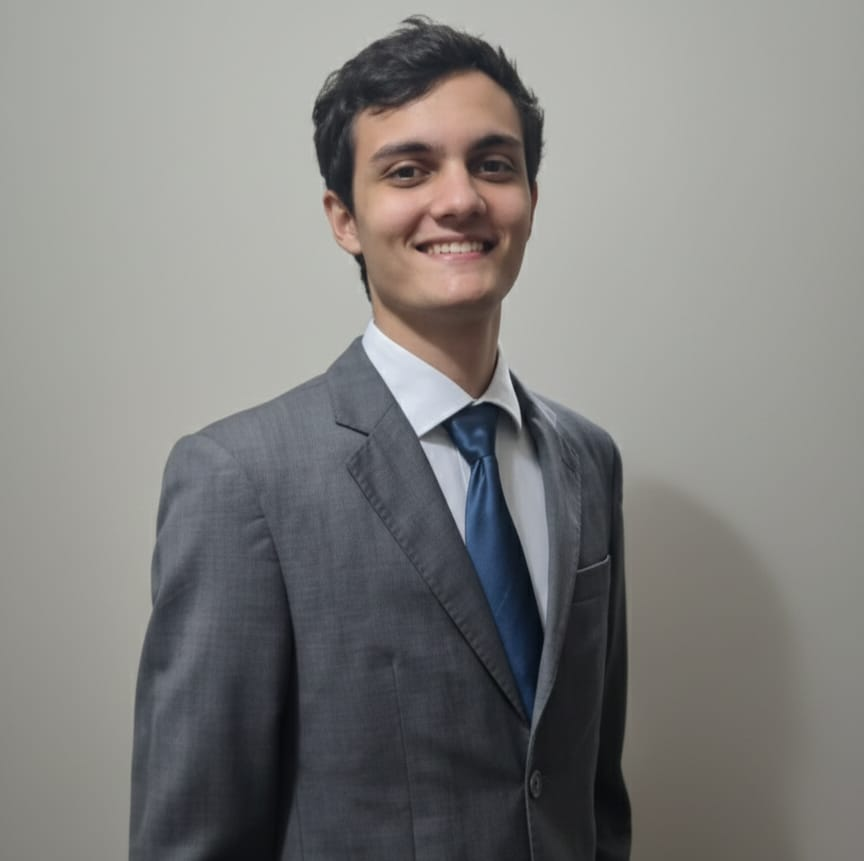
\includegraphics[width=\linewidth]{figuras/cap.jpeg}
\end{wrapfigure}

    \textbf{Pedro Consoli Bressan} é graduando em Engenharia da Computação pelo Instituto Nacional de Telecomunicações (Inatel), com previsão de conclusão em 2026. Atua no desenvolvimento de software, com experiência em aplicações web, mobile e sistemas embarcados, utilizando Python, C++, Java, TypeScript, React, Next.js, Node.js e Kotlin. Possui experiência internacional em projetos de tecnologia e participação em equipes de robótica, com atuação em desenvolvimento, automação e liderança técnica. Tem interesse em arquitetura de software, inteligência artificial, sistemas distribuídos e inovação tecnológica.
    \newline

\begin{wrapfigure}{l}{0.3\linewidth}
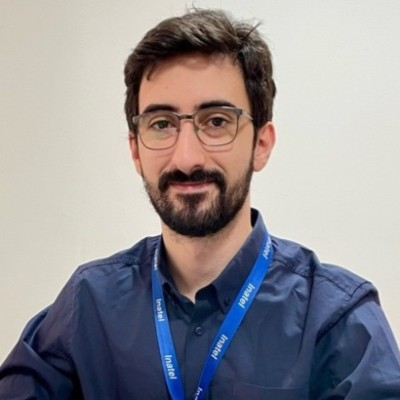
\includegraphics[width=\linewidth]{figuras/orientador.png}  
\end{wrapfigure}

   \textbf{Prof. MsC. Daniel Albino Mosca Rodrigues} é Engenheiro de Computação pelo Instituto Nacional de Telecomunicações (Inatel) e Mestre em Ciências da Computação pela Universidade Federal de Itajubá - Atua como professor e desenvolvedor de software e sistemas de baixo nível em C/C++.
